\documentclass[10pt,a4paper]{article}
\usepackage[utf8]{inputenc}
\usepackage[french]{babel}
\usepackage[T1]{fontenc}
\usepackage{graphicx}
\usepackage{listings}

\usepackage{fancyhdr}
\usepackage{vmargin}

\setlength{\parindent}{0cm}
\setlength{\parskip}{1ex plus 0.5ex minus 0.2ex}
\newcommand{\hsp}{\hspace{20pt}}
\newcommand{\HRule}{\rule{\linewidth}{0.5mm}}

\begin{document}
	\pagestyle{fancy}
	\fancyhf{}
	\rhead{SALEMI Marco, LECOCQ Alexis}
	\lhead{Pi randomness}
	\cfoot{\thepage}
	
	\begin{titlepage}
		\begin{center}
			% Upper part of the page. The '~' is needed because \\
			% only works if a paragraph has started.
			
\includegraphics[scale=1.5]{images/pi.png}~\\[1.5cm]
			
			% Title
			\HRule \\[0.5cm]
			{ \huge \bfseries Pi randomness\\[0.4cm] }
			\HRule \\[1.5cm]
			
			\Large{Rapport de projet de simulation}\\[2cm]
			
			\Large{Année académique 2016-2017}\\[2cm]
			
			% Author and supervisor
			\begin{minipage}{0.4\textwidth}
				\begin{flushleft} \large
					\emph{\textbf{Auteurs :}}\\
					SALEMI Marco\\
					LECOCQ Alexis
				\end{flushleft}
			\end{minipage}
			\begin{minipage}{0.4\textwidth}
				\begin{flushright} \large
					\emph{\textbf{Directeurs :}}\\
					BUYS Alain\\
					-\\
				\end{flushright}
			\end{minipage}
			
			\vfill
			
			% Bottom of the page
			{\large \today}
			
		\end{center}
	\end{titlepage}
	
	\newpage
	\tableofcontents
	
	\newpage
	\section{Introduction}
	Dans le cadre du cours de simulation, nous avons été amenés à réaliser un projet afin de mettre en pratique la théorie vue au cours.
	
	Les objectifs du projet sont :
	\begin{enumerate}
		\item analyser le caractère aléatoire des décimales de pi par des tests vus au cours ;
		\item utiliser ces décimales pour construire un générateur de loi uniforme dans l'intervalle [0, 1[ ;
		\item comparer le générateur du point 2 avec celui utilisé par défaut dans Python.
	\end{enumerate}
	
	Pour ce faire, un fichier nous est fourni. Celui-ci contient les 1 000 000 premières décimales du nombre pi.
	
	Le projet doit être réalisé en python et nous avons opté pour la version 3.

	Nous avons utilisé deux librairies externes :
	\begin{itemize}
		\item \textbf{scipy} : pour l'accès à la table des valeurs de Kolmogorov-Smirnov ;
		\item \textbf{plotly} : pour réaliser les graphiques.
	\end{itemize}
	
	L'installation de ces libraires est très simple à l'aide du gestionnaire de paquets pip3 :
	
	\begin{center}
		\begin{tabular}{|l|}
			\hline \\
			\$ pip3 install scipy plotly\\
			\\
			\hline
		\end{tabular}
	\end{center}
	
	Sur certains systèmes, les droits administrateurs sont requis pour installer ces librairies.
	
	\newpage
	\section{Les décimales de $\pi$}
	
	\subsection{Test de $\chi^2$}
	Le premier test consiste à étudier le nombre d'apparitions de chaque décimale. Si la séquence suit une loi uniforme, l'ensemble des décimales apparaissent exactement le même nombre de fois.
	
	
	Résultats du test :
	\begin{figure}[h]
		\centering
		\begin{tabular}{|r|r|r|}
			\hline
			Décimales & Valeur attendue & Valeur observée\\
			\hline
			0 & 100000 & 99959\\
			1 & 100000 & 99758\\
			2 & 100000 & 100026\\
			3 & 100000 & 100229\\
			4 & 100000 & 100230\\
			5 & 100000 & 100359\\
			6 & 100000 & 99548\\
			7 & 100000 & 99800\\
			8 & 100000 & 99985\\
			9 & 100000 & 100106\\
			\hline
		\end{tabular}
		\caption{Tableau des décimales}
	\end{figure}
	
	Graphique :
	\begin{figure}[h]
		\centering
		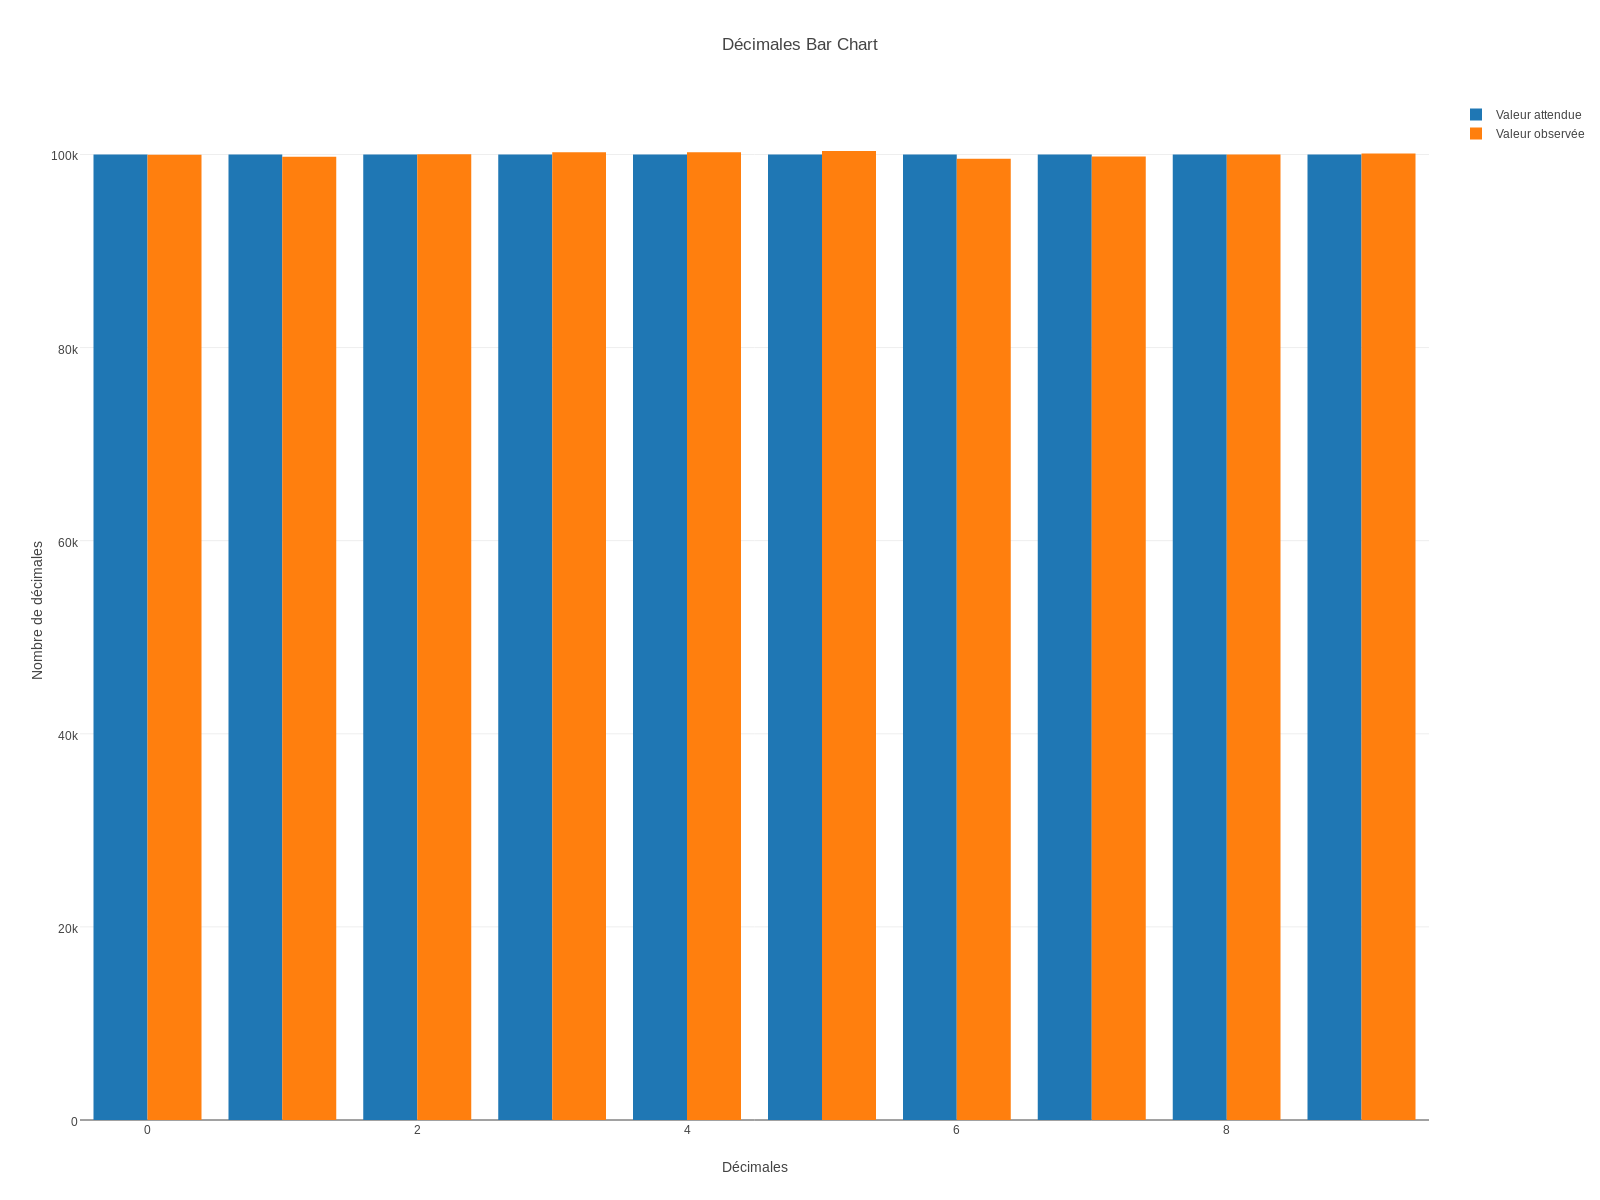
\includegraphics[scale=0.25]{../chart_images/decimales_bar_chart.png}
		\caption{Graphique des décimales}
	\end{figure}
	
	\newpage
	Test de $\chi^2$ :
	\begin{figure}[h]
		\centering
		\begin{tabular}{|r|r|r|r|}
			\hline
			$\alpha$ & Valeur & Limite & Résultat\\
			\hline
			0.001 & 5.509 & 27.877 & réussi\\
			0.01 & 5.509 & 21.666 & réussi\\
			0.05 & 5.509 & 16.919 & réussi\\
			0.1 & 5.509 & 14.684 & réussi\\
			\hline
		\end{tabular}
		\caption{Tableau du $\chi^2$}
	\end{figure}
	
	Comme nous pouvons le voir dans le tableau, le test est réussi pour tous les $\alpha$ choisis.
	
	\newpage
	\subsection{Test du poker}
	
	Le test du poker consiste à prendre une suite de décimales (ici 5) et calculer le nombre de décimales différentes qui composent cette suite. Si la séquence suit une loi uniforme, la probabilité d'avoir r chiffres différents dans une séquence de longueur l est :
	\[
		\frac{
			\left\{
				\begin{array}{l}
					l\\
					r\\
				\end{array}
			\right\}
			\prod_{i=10-r+1}^{10}i
		}{10^l}
	\]
	
	où $\left\{
	\begin{array}{l}
	l\\
	r\\
	\end{array}
	\right\}$ est le nombre de Stirling.
	
	Résultats du test :
	\begin{figure}[h]
		\centering
		\begin{tabular}{|r|r|r|}
			\hline
			Poker & Valeur attendue & Valeur observée\\
			\hline
			1 & 20 & 13\\
			2 & 2700 & 2644\\
			3 & 36000 & 36172\\
			4 & 100800 & 100670\\
			5 & 60480 & 60501\\
			\hline
		\end{tabular}
		\caption{Tableau du Poker}
	\end{figure}
	
	Graphique :
	\begin{figure}[h]
		\centering
		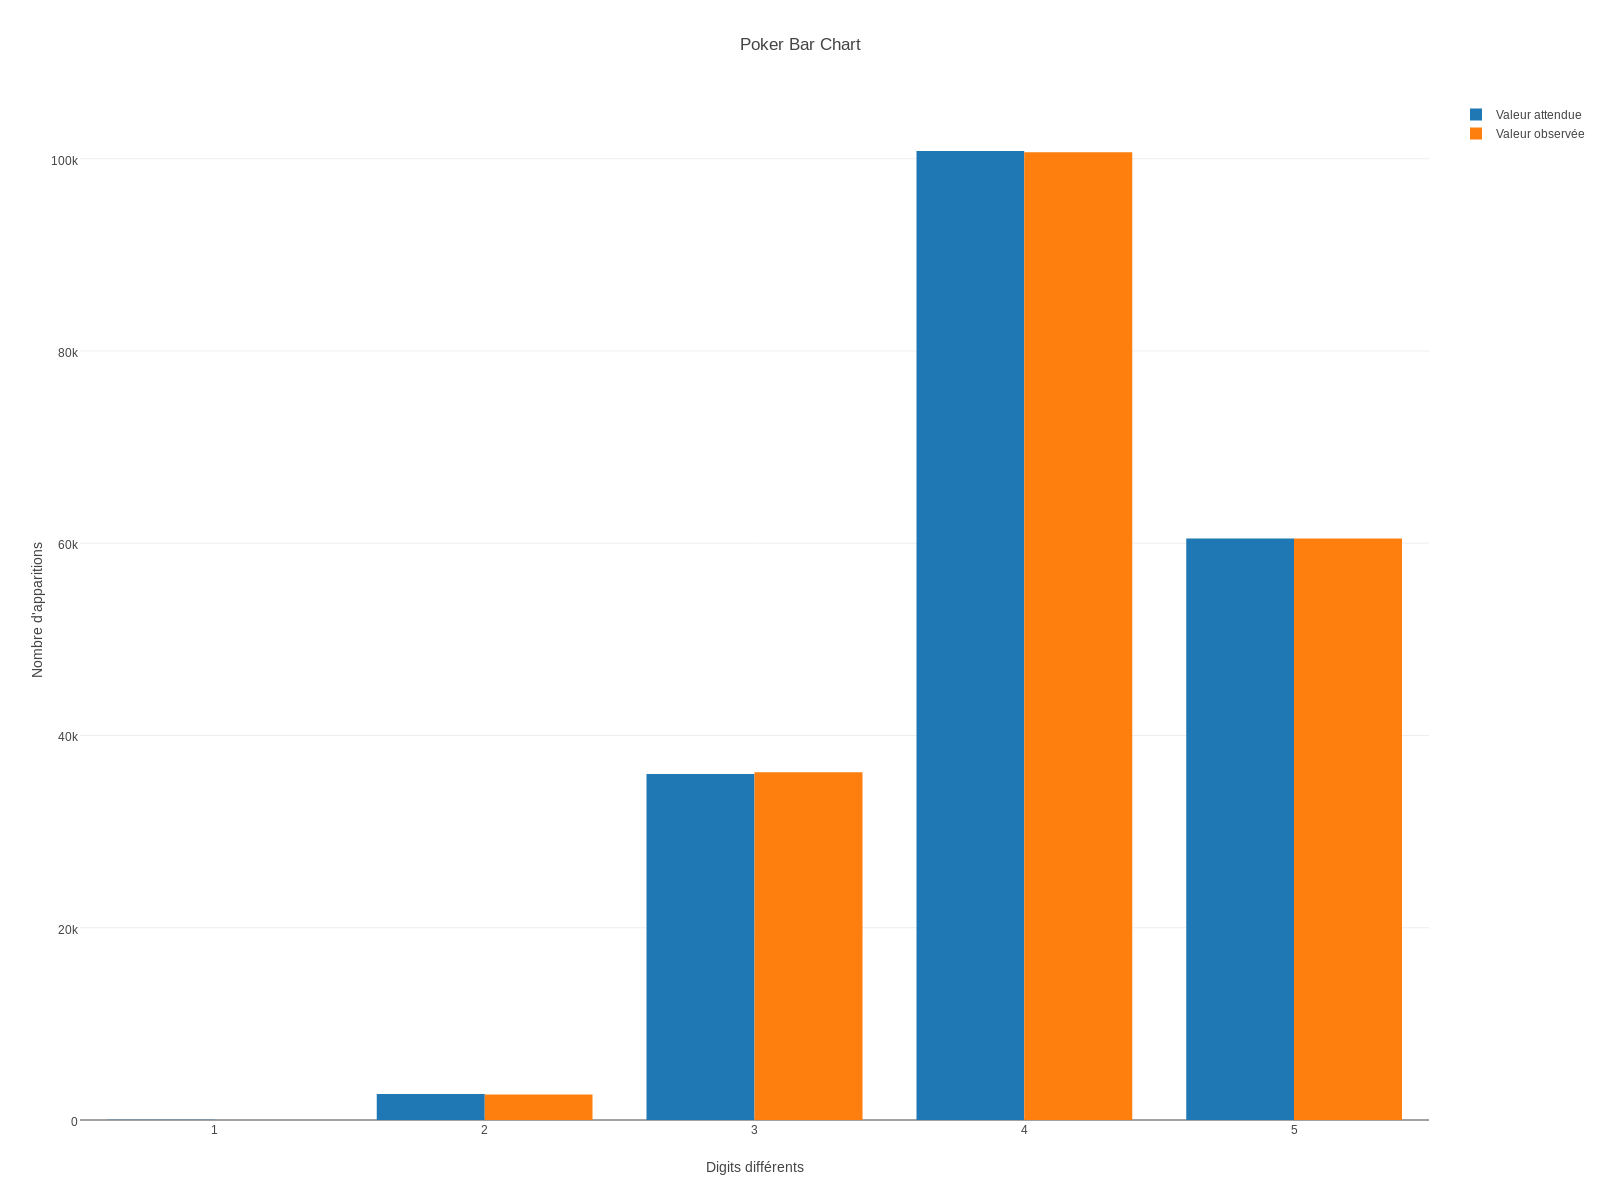
\includegraphics[scale=0.25]{../chart_images/poker_bar_chart.png}
		\caption{Graphique du Poker}
	\end{figure}
	
	\newpage
	Test de $\chi^2$ :
	\begin{figure}[h]
		\centering
		\begin{tabular}{|r|r|r|r|}
			\hline
			$\alpha$ & Valeur & Limite & Résultat\\
			\hline
			0.001 & 4.608 & 18.467 & réussi\\
			0.01 & 4.608 & 13.277 & réussi\\
			0.05 & 4.608 & 9.488 & réussi\\
			0.1 & 4.608 & 7.779 & réussi\\
			\hline
		\end{tabular}
		\caption{Tableau du $\chi^2$}
	\end{figure}
	
	Comme nous pouvons le voir dans le tableau, le test est réussi pour tous les $\alpha$ choisis.	
		
\newpage
	
\subsection{Test du collectionneur de coupons}
Le collectionneur de coupons est un test permettant de vérifier si nos différentes décimales de Pi suivent une loi uniforme.
 
Le fonctionnement de ce test que nous avons adapté à notre problème se déroule comme ceci:  
\begin{itemize}
\item Nous parcourons les différentes décimales de Pi dans l'ordre, en calculant le nombres de digits visités.
\item Lorsque nous avons rencontrés tous les différents digits (de 0 à 9) dans une séquence donnée de taille r, nous gardons la valeur r en mémoire.
\item Nous recommençons ensuite le procédé avec les décimales qui suivent 
\end{itemize}

Nous obtenons ainsi les différentes occurrences de séquences de tailles $r_i$ contenant tout les différents digits.

Nous comparons ensuite cette valeur à la valeur théorique suivant une loi uniforme, et ceci à l'aide d'un $\chi^2$.

Nous calculons la valeur théorique à l'aide de la probabilité $ S_r$ ci-dessous. Celle-ci représente la probabilité de rencontrer r digits avant d'avoir rencontré tout les différents digits possibles. r est donc la longueur de la séquence contenants les digits.

\begin{figure}[h]
		\centering
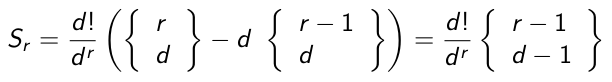
\includegraphics[scale=0.4]{images/formule.png}  
\caption{Graphique du Poker}
	\end{figure}

\textbf{où} d est le nombre de différents digits possibles (il vaut 10 dans notre cas)

\textbf{Remarque :} $S_r$ sera égal à 0 lorsque r<d, donc lorsque r<10.

 

Ceci s'explique par le fait qu'il est impossible de rencontrer tout les différents digits, puisque la séquence est plus petite que le nombre des digits (qui vaut ici 10). 

Nous obtenons donc le tableau de valeurs suivant pour les différentes longueurs de séquences , ainsi que le graphique correspondant, et le tableau représentant nos tests de $\chi^2$. .

\newpage

\begin{figure}[h]
		\centering
\begin{tabular}{|r|r|r|}
\hline
Collectionneur de coupons & Valeur attendue & Valeur observée\\
\hline
0-9 & 0 & 0\\
10 & 12.39307776 & 12\\
11 & 55.76884992 & 62\\
12 & 143.140048128 & 154\\
13 & 276.055807104 & 265\\
14 & 445.533624088 & 496\\
15 & 636.400653977 & 645\\
16 & 831.928596481 & 869\\
17 & 1017.20430344 & 1008\\
18 & 1180.91435762 & 1150\\
19 & 1315.83993579 & 1341\\
20 & 1418.52980752 & 1354\\
... & ... & ...\\
45 & 314.649867464 & 324\\
46 & 284.820911145 & 280\\
47 & 257.651373497 & 266\\
48 & 232.938892283 & 219\\
49 & 210.488959104 & 212\\
50 & 190.116510903 & 185\\
51 & 171.646916633 & 197\\
52 & 154.916499868 & 142\\
53 & 139.772710642 & 148\\
54 & 126.074036915 & 115\\
55 & 113.689727286 & 113\\
... & ... & ...\\
90 & 2.88994755473 & 0\\
91 & 2.60102568515 & 1\\
92 & 2.34098142576 & 4\\
93 & 2.10692993077 & 4\\
94 & 1.89627425595 & 0\\
95 & 1.7066766851 & 1\\
96 & 1.53603290049 & 1\\
97 & 1.38244871762 & 4\\
98 & 1.24421913165 & 0\\
99 & 1.11980944715 & 2\\
100 & 1.0078382854 & 0\\
101 & 0.907062283239 & 1\\
\hline
\end{tabular}
\caption{Tableau du Collectionneur De Coupons 2}
	\end{figure}

\newpage

\begin{figure}[h]
		\centering
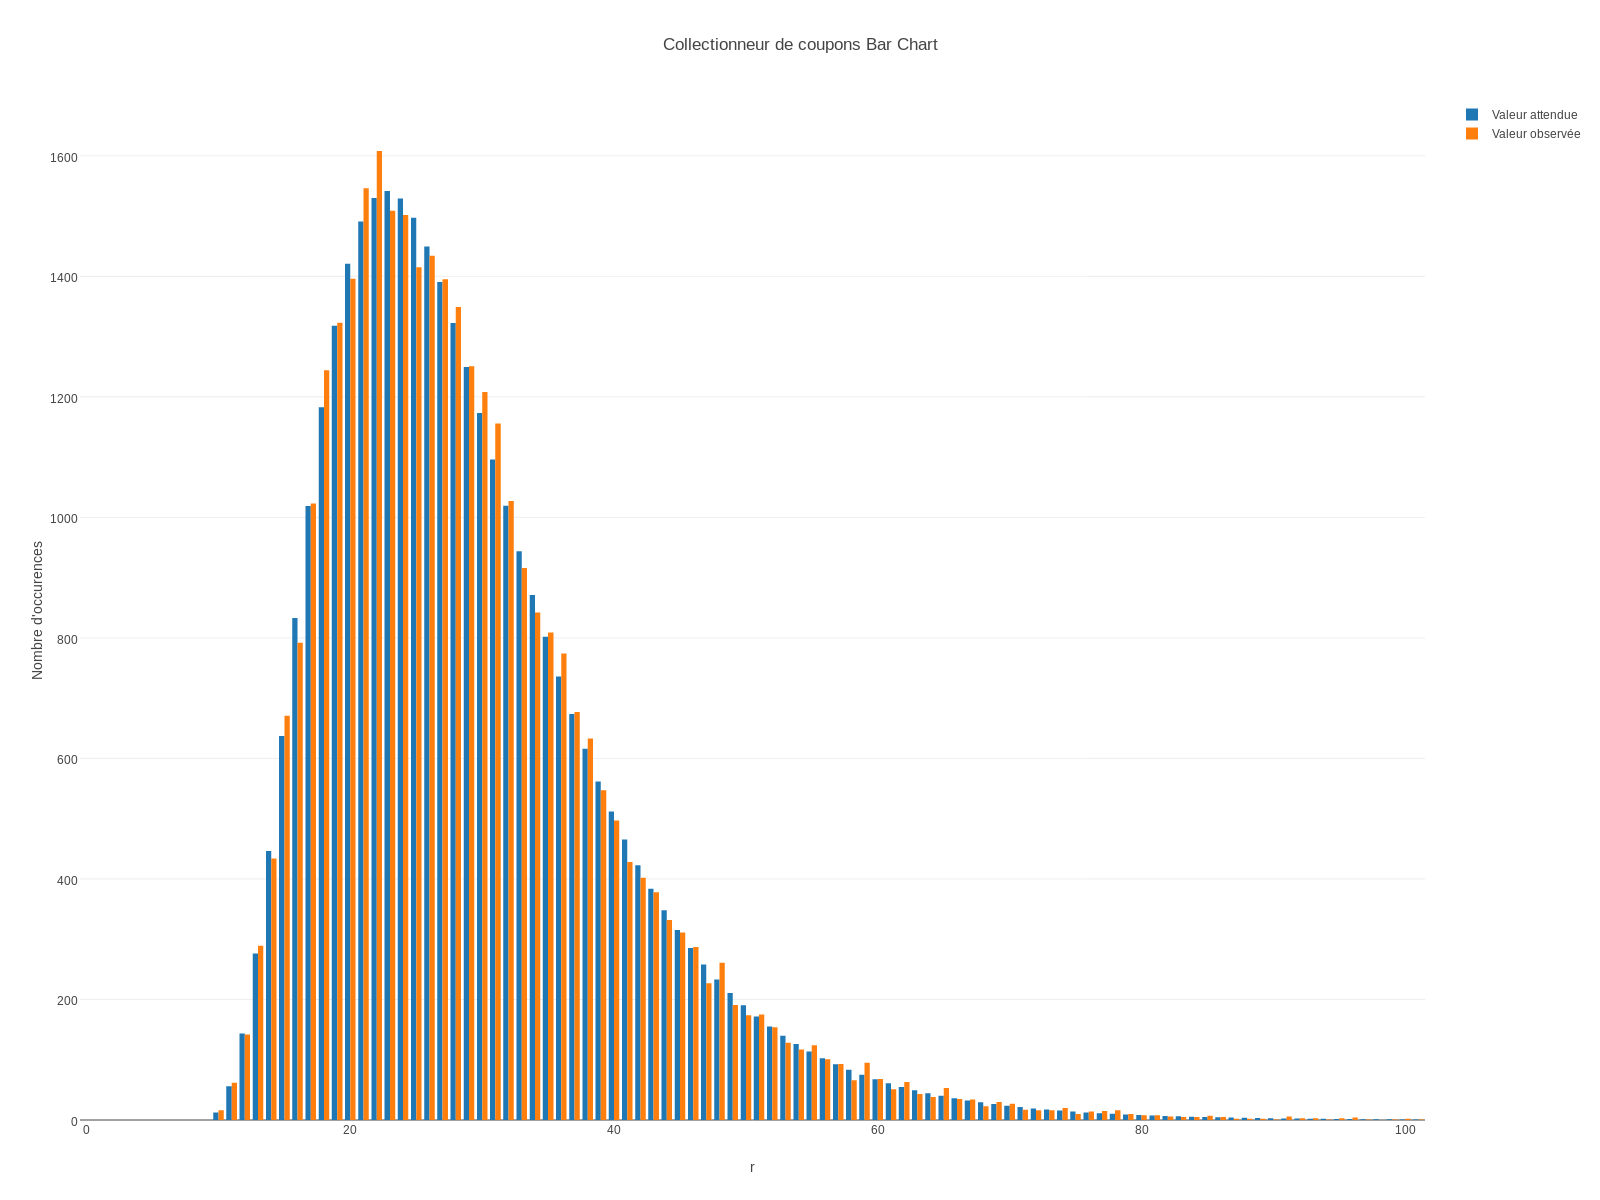
\includegraphics[scale=0.25]{../chart_images/collectionneur_de_coupons_bar_chart.png}
\caption{Graphique du Collectionneur De Coupons}
	\end{figure}

\begin{figure}[h]
		\centering
\begin{tabular}{|r|r|r|r|}
\hline
$\alpha$ & AValeur & Limite & Résultat\\
\hline
0.001 & 79.837 & 150.667055668 & réussi\\
0.01 & 79.837 & 136.971003847 & réussi\\
0.05 & 79.837 & 125.458419408 & réussi\\
0.1 & 79.837 & 119.588667243 & réussi\\
\hline
\end{tabular}
\caption{Tableau de $\chi^2$}
	\end{figure}
Nous remarquons que les valeurs du tableau sont proches des valeurs théoriques. Ainsi que notre graphique suit la forme d'une gaussienne. 

Ce test confirme donc que les décimales de Pi suivent bien une loi uniforme, car les différents tests de $\chi^2$ sont respectés.

\newpage
\subsection{Interprétation des résultats}
D'après les tests effectués ci-dessus, les décimales de pi suivent une loi uniforme.
	
	\newpage
	\section{Générateur de loi uniforme à partir des décimales de $\pi$}
	Notre générateur est très simple, il suit ces étapes :
	\begin{enumerate}
		\item lecture des $n$ premiers chiffres à l'emplacement actuel comme un nombre ;
		\item division de ce nombre par $10^{n}$ afin d'obtenir un nombre dans l'intervalle $[0, 1[$.
	\end{enumerate}
	Les caractères éventuellement manquants à la fin du fichiers sont lus en début de fichier. Ainsi, le générateur ne s'arrête jamais.
	
	Afin que le générateur ne commence pas toujours la séquence au même emplacement, nous choisissons l'emplacement de départ en fonction d'un timestamp.
	Ce timestamp représente le nombre de millisecondes écoulées depuis le 1er janvier 1970 UTC.
	
	Notre générateur possédant un paramètre $n$, sa période est variable.
	
	\subsection{Choix du paramètre}
	Paramétrer notre générateur soulève une question : quel paramètre utiliser par défaut et pourquoi ?
	
	Choisir un paramètre trop petit réduirait la précision du générateur.
	Par exemple si un seul digit est lu, alors il est évident que notre générateur ne générera que 10 nombres différents.
	Afin d'obtenir la meilleure précision possible, nous nous sommes fixé un minimum de 15 digits.
	Cela correspond à la précision utilisée par Python pour représenter u nombre flottant.
	Augmenter $n$ au-delà de 15 n'améliorerait donc pas la précision.
	
	Par ailleurs, choisir un paramètre qui divise 1000000 réduirait la période.
	Par exemple, si nous choisissons un paramètre de 100, alors il est évident qu'après 10000 générations, nous nous retrouverions au début du fichier.
	Cela réduirait la période à 10000.
	En fait, il convient d'utiliser un nombre qui est premier par rapport à 1000000 pour obtenir la période maximale de 1000000.
	
	Notre premier choix s'est donc porté sur le nombre $n = 17$, qui est le premier nombre premier après 15.
	Nous avons également réalisé différents tests pratiques et ce choix du paramètre s'est avéré le plus judicieux.
	Afin de ne pas perturber le lecteur, nous n'avons pas inclus les tests des autres paramètres dans ce rapport.
	Cependant, ces derniers sont facilement réalisables à l'aide du code fourni en annexe.
	
	\newpage
	\section{Comparaison avec le générateur par défaut de Python}
	Nous allons maintenant comparer le caractère aléatoire de notre générateur avec celui utilisé par défaut dans Python (Mersenne Twister).
	Nous n'allons pas réutiliser ni le test du $\chi^2$ ni le test du poker.
	Bien qu'il existe des méthodes de correspondance, d'autres tests sont plus appropriés pour tester des fonctions continues.
	Dans ces tests se trouve notamment le test de Kolmogorov-Smirnov.
	
	\newpage
	\subsection{Test de Kolmogorov-Smirnov}
	Le test de Kolmogorov-Smirnov est un test vérifiant si les valeurs générées pseudo-aléatoirement sont réparties uniformément entre 0 et 1.
	
	Pour effectuer ce test, nous générons 100 000 nombres avec notre générateur ainsi que 100 000 nombres avec le générateur de Python.
	Ensuite, nous divisons l'intervalle [0, 1] en 100 valeurs réparties uniformément.
	Pour chaque valeur, nous analysons la proportion de nombres de chaque générateur se trouvant en dessous de cette valeur.
	Nous comparons la proportion de chaque générateur avec la proportion attendue d'une loi uniforme et nous en prenons le plus grand écart ($D_n$).
	
	À l'aide de la table de Kolmogorov-Smirnov, nous pouvons accepter ou refuser l'hypothèse disant que les générateurs suivent une loi uniforme.
	
	Nous pouvons également aller plus loin et comparer les $D_n$ obtenus pour chaque générateur
	 Il est évident que le générateur ayant le plus petit $D_n$ sera celui se rapprochant d'avantage de la loi uniforme.
	\begin{figure}[h]
		\centering
		\begin{tabular}{|r|r|r|r|}
			\hline
			X & Valeurs attendues & Valeurs de Pi & Valeurs de Python\\
			\hline
			0.01 & 0.01 & 0.01008 & 0.01019\\
			0.02 & 0.02 & 0.02001 & 0.02041\\
			0.03 & 0.03 & 0.03026 & 0.03055\\
			0.04 & 0.04 & 0.03993 & 0.04118\\
			0.05 & 0.05 & 0.04986 & 0.05164\\
			0.06 & 0.06 & 0.05944 & 0.06145\\
			0.07 & 0.07 & 0.06959 & 0.07172\\
			0.08 & 0.08 & 0.0794 & 0.08185\\
			0.09 & 0.09 & 0.08891 & 0.09194\\
			0.1 & 0.1 & 0.09909 & 0.10154\\
			... & ... & ... & ...\\
			0.45 & 0.45 & 0.44995 & 0.45082\\
			0.46 & 0.46 & 0.4601 & 0.46057\\
			0.47 & 0.47 & 0.47026 & 0.47057\\
			0.48 & 0.48 & 0.48063 & 0.48064\\
			0.49 & 0.49 & 0.49032 & 0.49075\\
			0.5 & 0.5 & 0.50059 & 0.50101\\
			0.51 & 0.51 & 0.51073 & 0.51043\\
			0.52 & 0.52 & 0.52031 & 0.52009\\
			0.53 & 0.53 & 0.53065 & 0.53072\\
			0.54 & 0.54 & 0.54064 & 0.54095\\
			0.55 & 0.55 & 0.55076 & 0.55057\\
			... & ... & ... & ...\\
			0.9 & 0.9 & 0.8998 & 0.90023\\
			0.91 & 0.91 & 0.90979 & 0.91049\\
			0.92 & 0.92 & 0.91907 & 0.92049\\
			0.93 & 0.93 & 0.92897 & 0.93025\\
			0.94 & 0.94 & 0.93927 & 0.94029\\
			0.95 & 0.95 & 0.94987 & 0.95097\\
			0.96 & 0.96 & 0.95941 & 0.96029\\
			0.97 & 0.97 & 0.96985 & 0.96935\\
			0.98 & 0.98 & 0.9798 & 0.97962\\
			0.99 & 0.99 & 0.98989 & 0.98957\\
			\hline
		\end{tabular}
	\caption{Tableau de Kolmogorov-Smirnov}
	\end{figure}
	
	\begin{figure}[h]
		\centering
		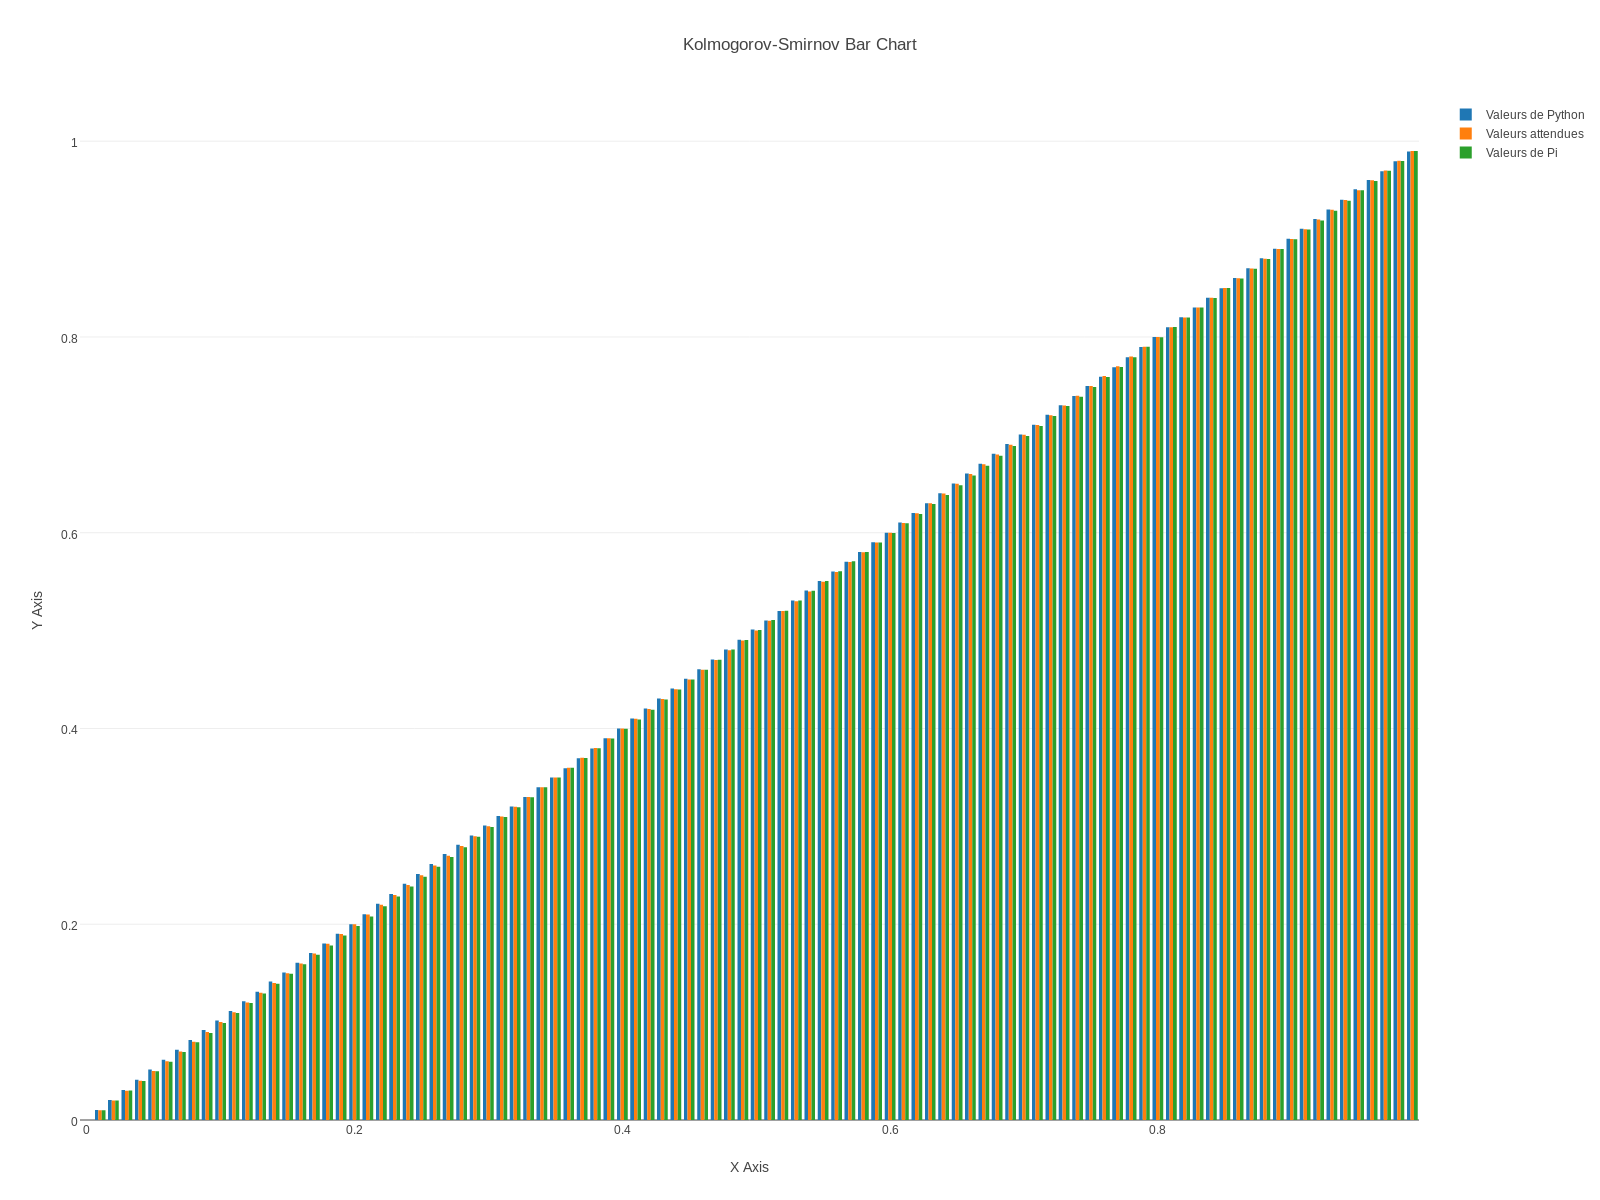
\includegraphics[scale=0.25]{../chart_images/kolmogorov-smirnov_bar_chart.png}
		\caption{Graphique de Kolmogorov-Smirnov}
	\end{figure}
	
	\begin{figure}[h]
		\centering
		\begin{tabular}{|r|r|r|r|r|}
			\hline
			$\alpha$ & Valeur Pi & Valeur Python & Limite & Meilleur\\
			\hline
			0.001 & 0.00212 & 0.00194 & 0.006165 & Python\\
			0.01 & 0.00212 & 0.00194 & 0.005147 & Python\\
			0.05 & 0.00212 & 0.00194 & 0.004295 & Python\\
			0.1 & 0.00212 & 0.00194 & 0.00387 & Python\\
			\hline
		\end{tabular}
		\caption{Tableau des $D_\alpha$}
	\end{figure}
	
	\newpage
	Nous remarquons que le générateur de Python est meilleur dans ce test.
	Cependant, si on répète ce test, il est possible d'obtenir des résultats différents.
	En effet, tant que le nombre de nombres générés sera inférieur au plus petit commun multiple entre la période des deux générateurs, nous obtiendrons des nombres et donc des résultats différents.
	
	
\newpage
\subsection{Test du gap}
Le test du gap est un test vérifiant la grandeur des trous (gap en anglais) séparant des nombres faisant partie d'un même intervalle.

Ce test se fait en différentes étapes:
\begin{itemize}
\item Nous générons n nombres à travers nos générateurs de nombres aléatoires.
\item Nous choisissons un intervalle $[a,b]\in[0,1]$ (nous avons ici choisis a=0 et b =1/2 pour un temps de calcul optimal).
\item Nous marquons les nombres se trouvant dans cet intervalle
\item Nous calculons les distances entre chaque nombres marqués (nous notons $r_i$ les différentes distances. 
\end{itemize} 

Nous obtenons ainsi les différentes occurrences $r_i$ que nous appelons les gaps (trous en anglais), et pouvons les comparer à l'aide d'un $\chi^2$ avec les valeurs théoriques attendues :

\[
	r_i = N p (1-p)^i
\] 
\[
	r_{>i} = N (1-p)^{i+1}
\]

où N est le nombres total de gaps observés

p est la probabilité d'être dans l'intervalle $|b-a|$


Nous avons donc effectuer ce test sur notre générateur pseudo-aléatoire et le générateur de python.

	\subsubsection{Notre générateur}

Ci-dessous nous avons illustrer les occurrences pour les différents gaps obtenus dans un tableau et à l'aide d'un graphique. 
Nous avons fixé la limite à 15 afin d'éviter les classes vides, ces dernières étant néfastes au test de $\chi^2$.

\begin{figure}[h]
	\centering
	\begin{tabular}{|r|r|r|}
		\hline
		APi Gap & Valeur attendue & Valeur observée\\
		\hline
		0 & 250101.000 & 250067\\
		1 & 125050.500 & 125248\\
		2 & 62525.250 & 62273\\
		3 & 31262.625 & 31471\\
		4 & 15631.312 & 15616\\
		5 & 7815.656 & 7860\\
		6 & 3907.828 & 3826\\
		7 & 1953.914 & 1898\\
		8 & 976.957 & 954\\
		9 & 488.479 & 471\\
		10 & 244.239 & 252\\
		11 & 122.120 & 135\\
		12 & 61.060 & 66\\
		13 & 30.530 & 30\\
		14 & 15.265 & 19\\
		> 15 & 15.265 & 16\\
		\hline
		Total & 500202 & 500202\\
		\hline
	\end{tabular}
	\caption{Tableau de Pi Gap}
\end{figure}

\begin{figure}[h]
\centering
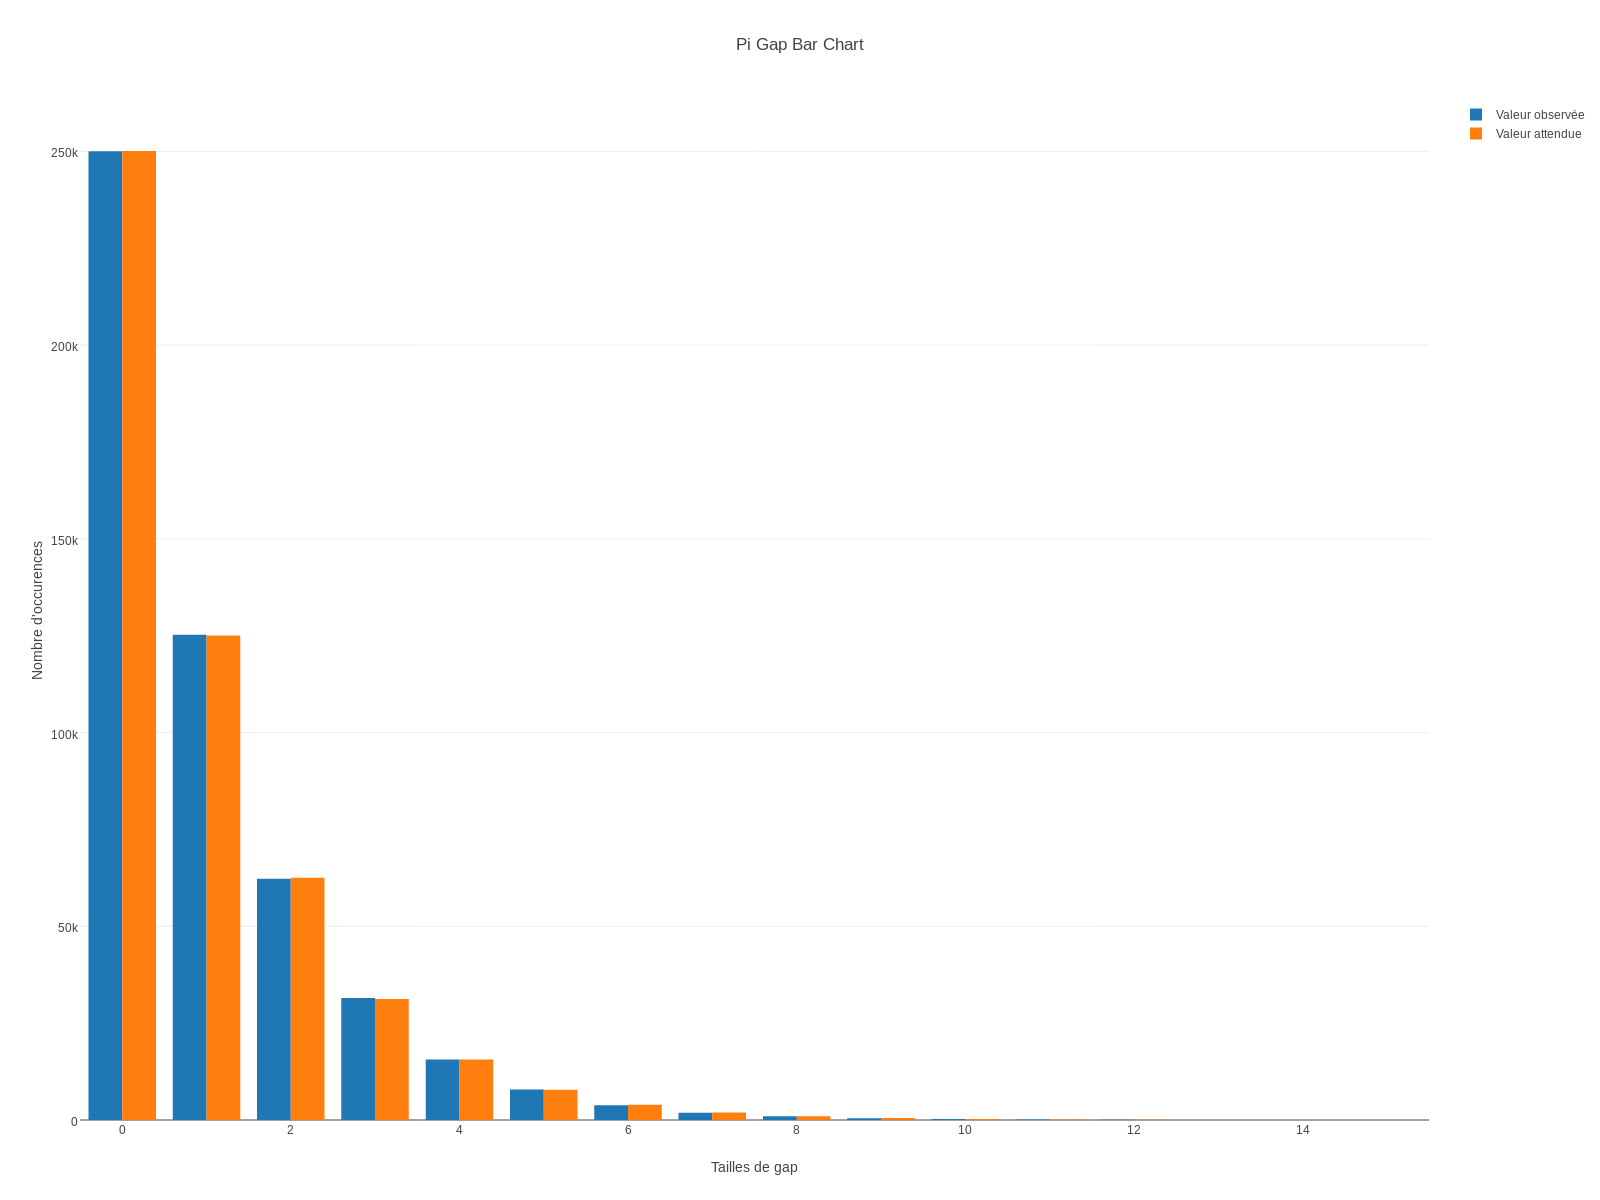
\includegraphics[scale=0.25]{../chart_images/pi_gap_bar_chart.png}
\caption{Graphique de Gap}
\end{figure}
\newpage

Résultats du test de $\chi^2$ :
\begin{figure}[h]
	\centering
	\begin{tabular}{|r|r|r|r|}
		\hline
		$\alpha$ & AValeur & Limite & Résultat\\
		\hline
		0.001 & 10.431 & 37.697 & réussi\\
		0.010 & 10.431 & 30.578 & réussi\\
		0.050 & 10.431 & 24.996 & réussi\\
		0.100 & 10.431 & 22.307 & réussi\\
		\hline
	\end{tabular}
	\caption{Tableau de $\chi^2$}
\end{figure}


Nous constatons donc que les différentes valeurs observées sont proches des valeurs théoriques. Et que le test de $\chi^2$ réussit bien. Notre générateur passe donc ce test avec succès.

\newpage

	\subsubsection{Le générateur de python}
En ce qui concerne ce générateur, nous avons procédé de la même façon que ci-dessus pour notre générateur.
	
\begin{figure}[h]
	\centering
	\begin{tabular}{|r|r|r|}
		\hline
		APython Gap & Valeur attendue & Valeur observée\\
		\hline
		0 & 249672.000 & 249152\\
		1 & 124836.000 & 125037\\
		2 & 62418.000 & 62606\\
		3 & 31209.000 & 31237\\
		4 & 15604.500 & 15686\\
		5 & 7802.250 & 7839\\
		6 & 3901.125 & 3834\\
		7 & 1950.562 & 1969\\
		8 & 975.281 & 942\\
		9 & 487.641 & 522\\
		10 & 243.820 & 254\\
		11 & 121.910 & 122\\
		12 & 60.955 & 78\\
		13 & 30.478 & 31\\
		14 & 15.239 & 19\\
		> 15 & 15.239 & 16\\
		\hline
		Total & 499344 & 499344\\
		\hline
	\end{tabular}
	\caption{Tableau de Python Gap}
\end{figure}

\begin{figure}[h]
\centering
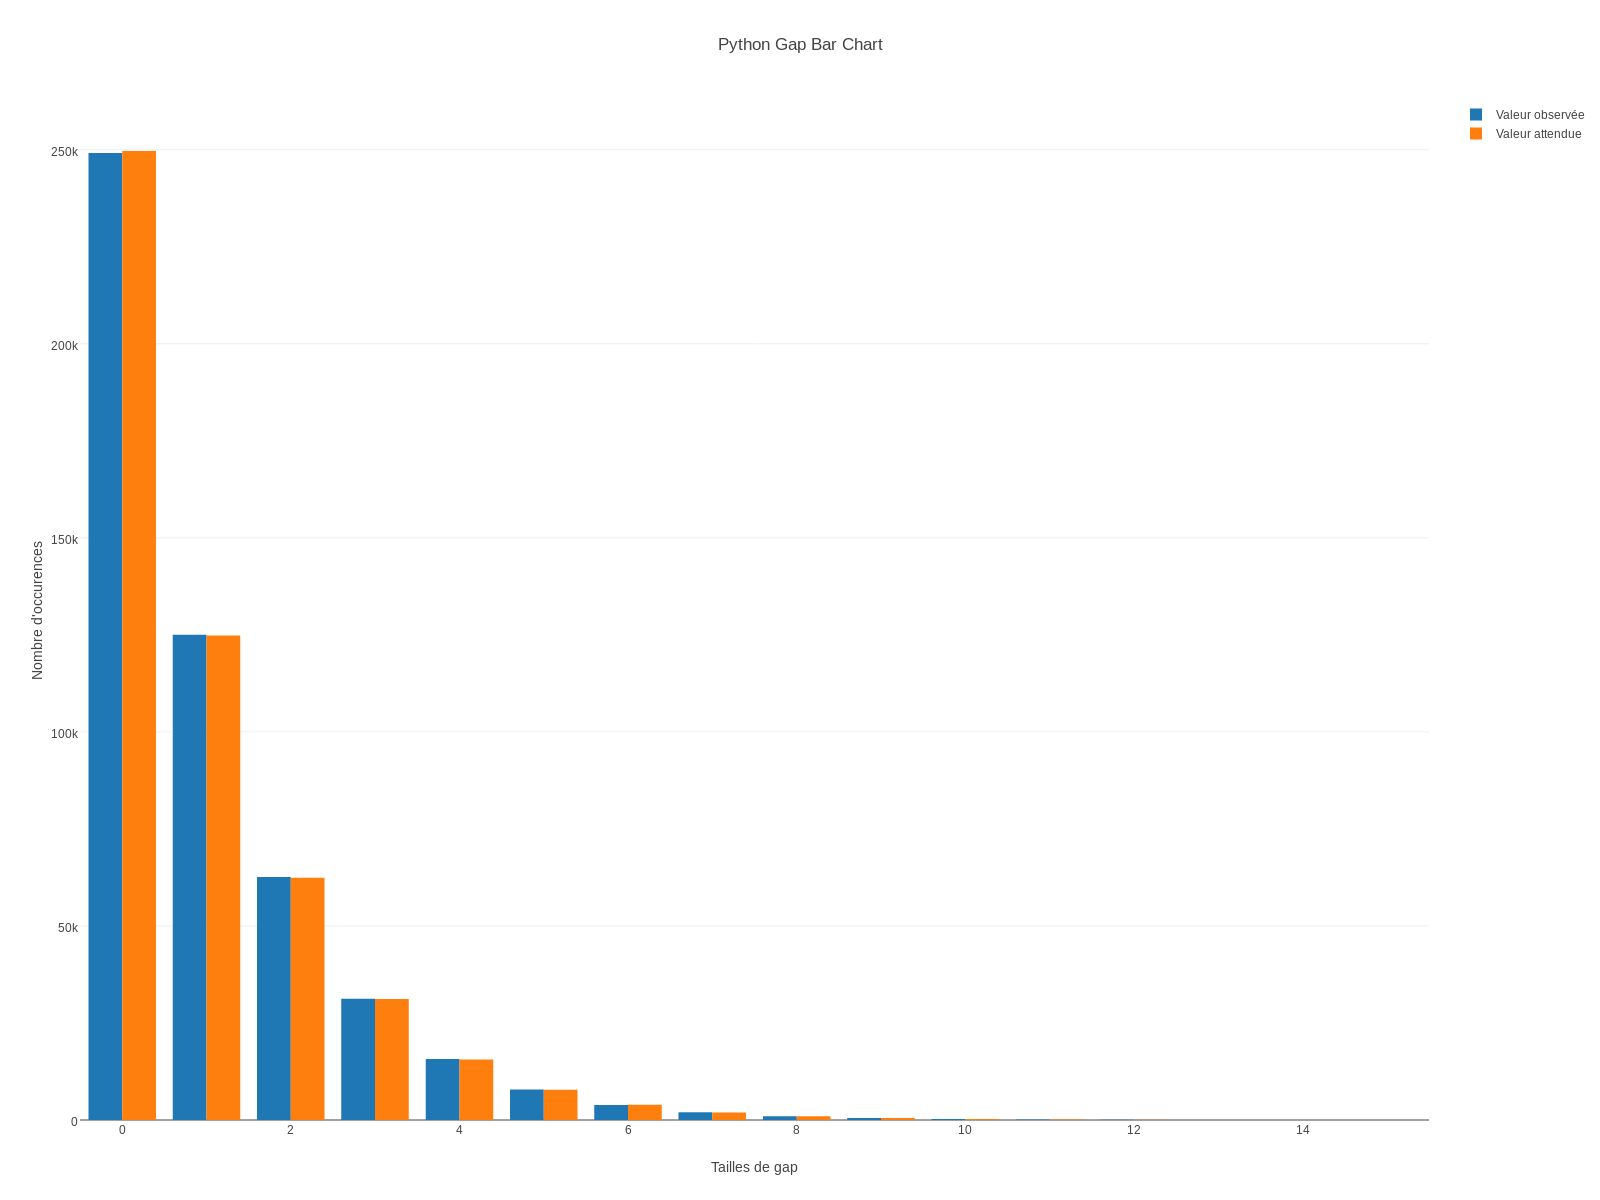
\includegraphics[scale=0.20]{../chart_images/python_gap_bar_chart.png}
\caption{Graphique de Gap}
\end{figure}

\begin{figure}[h]
	\centering
	\begin{tabular}{|r|r|r|r|}
		\hline
		$\alpha$ & AValeur & Limite & Résultat\\
		\hline
		0.001 & 13.649 & 37.697 & réussi\\
		0.010 & 13.649 & 30.578 & réussi\\
		0.050 & 13.649 & 24.996 & réussi\\
		0.100 & 13.649 & 22.307 & réussi\\
		\hline
	\end{tabular}
	\caption{Tableau de $\chi^2$}
\end{figure}


\newpage

Nous observons, ici aussi, que les valeurs sont proches des valeurs théoriques et que le test de $\chi^2$  est réussi.

\newpage

\subsection{Le collectionneur de coupons}

Tout comme nous l'avons précédemment effectué sur les décimales de Pi, nous allons ici effectuer le même test sur le générateur de python.

Afin d'effectuer ce test comme précédemment, nous avons du avoir recourt à une petite adaptation. 

Nous avons donc discrétiser 1 million de nombres générés aléatoirement par python entre 0 et 1. Nous avons choisis ce nombre en rapport avec notre notre nombre de Pi qui possède 1 million de décimales.

Nous obtenons donc le tableau de valeurs, le graphique associé et les test de $\chi^2$ suivants :

 \begin{figure}[h]
\centering
\begin{tabular}{|r|r|r|}
\hline
Collectionneur de coupons & Valeur attendue & Valeur observée\\
\hline
0-9 & 0 & 0\\
10 & 12.40614144 & 7\\
11 & 55.82763648 & 59\\
12 & 143.290933632 & 151\\
13 & 276.346800576 & 268\\
14 & 446.003265996 & 462\\
15 & 637.071490928 & 643\\
16 & 832.805541594 & 810\\
17 & 1018.27654972 & 1016\\
18 & 1182.15917248 & 1166\\
19 & 1317.22697718 & 1336\\
20 & 1420.02509544 & 1436\\
... & ... & ...\\
45 & 314.98154336 & 300\\
46 & 285.12114401 & 307\\
47 & 257.922966653 & 258\\
48 & 233.18443574 & 219\\
49 & 210.710837838 & 198\\
50 & 190.316914815 & 194\\
51 & 171.827851541 & 157\\
52 & 155.07979906 & 163\\
53 & 139.920046598 & 127\\
54 & 126.206932948 & 127\\
55 & 113.809568882 & 121\\
... & ... & ...\\
... & ... & ...\\
90 & 2.89299388033 & 3\\
91 & 2.60376745503 & 2\\
92 & 2.34344908011 & 3\\
93 & 2.10915086885 & 1\\
94 & 1.89827313956 & 2\\
95 & 1.70847571183 & 2\\
96 & 1.53765204971 & 1\\
97 & 1.38390597207 & 3\\
98 & 1.24553067677 & 0\\
99 & 1.12098985065 & 1\\
100 & 1.00890065885 & 0\\
101 & 0.9080184276 & 0\\
\hline
\end{tabular}
\caption{Tableau de Collectionneur de coupons 2}
\end{figure}

\begin{figure}[h]
\centering
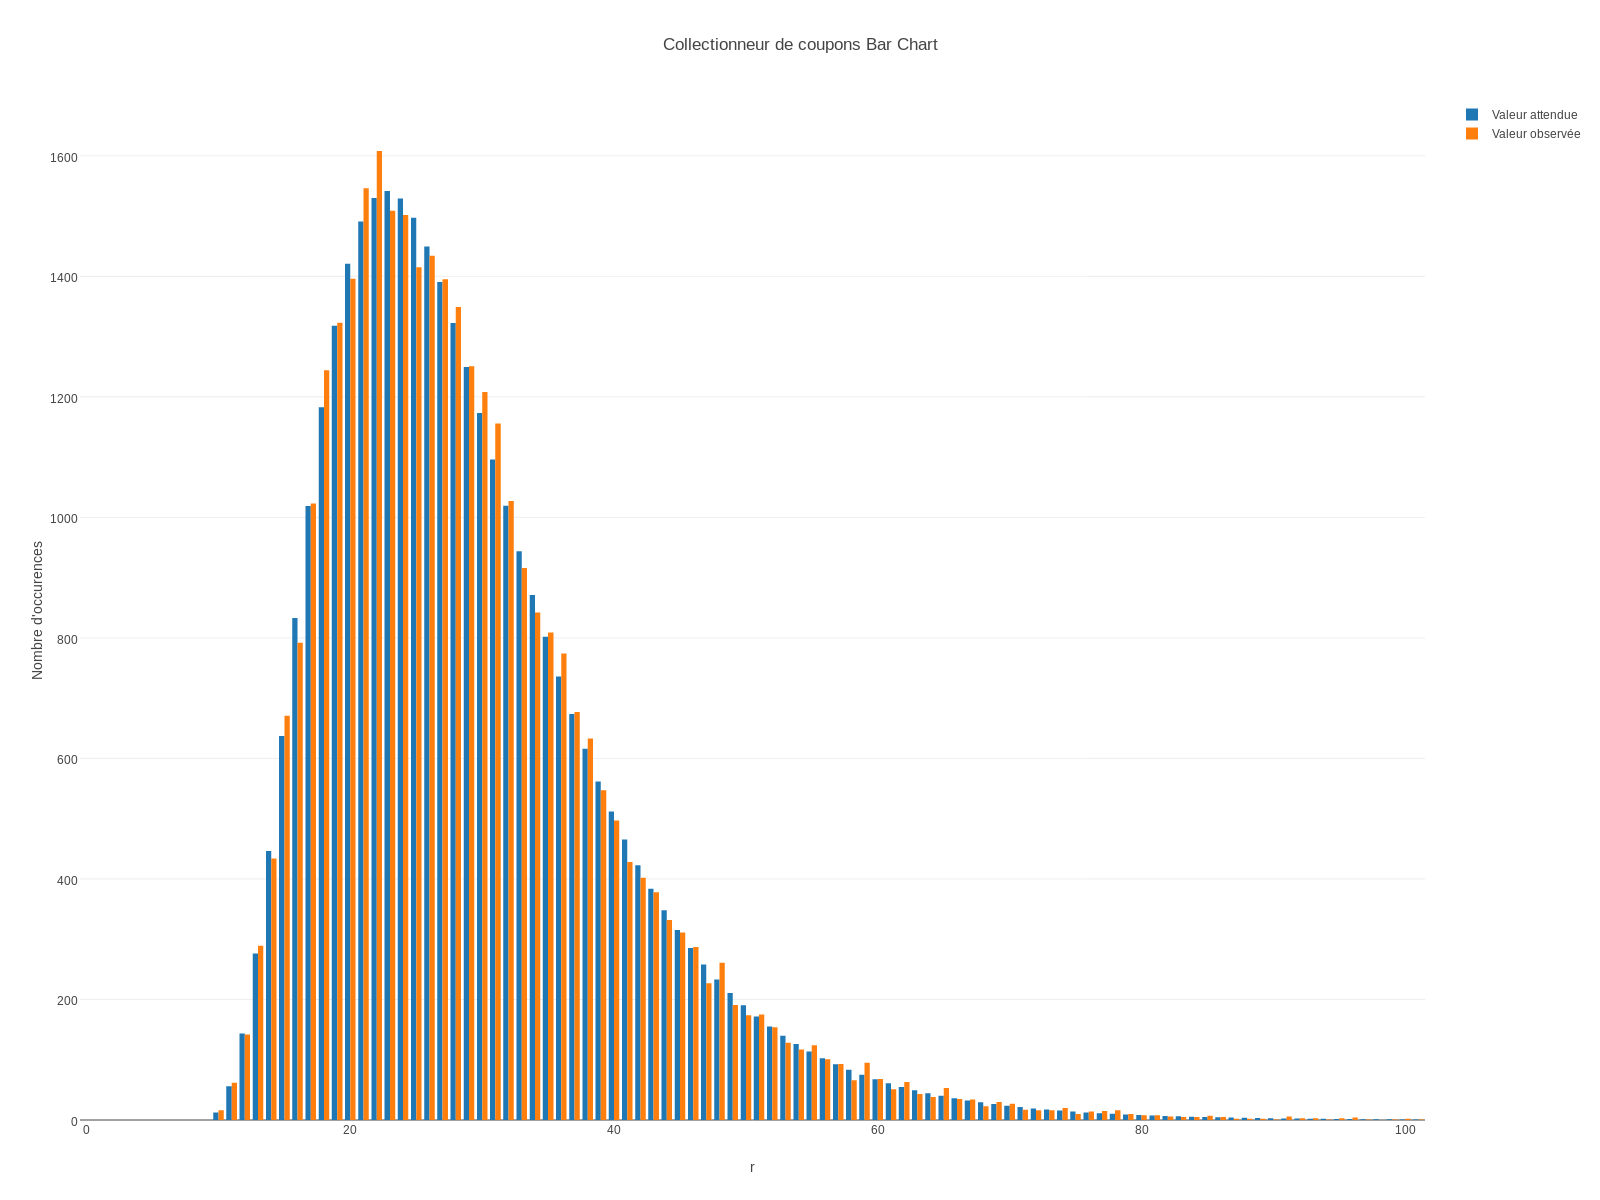
\includegraphics[scale=0.25]{../chart_images/collectionneur_de_coupons_bar_chart.png}
\end{figure}

\begin{figure}[h]
\centering
\begin{tabular}{|r|r|r|r|}
\hline
$\alpha$ & AValeur & Limite & Résultat\\
\hline
0.001 & 70.467 & 150.667055668 & réussi\\
0.01 & 70.467 & 136.971003847 & réussi\\
0.05 & 70.467 & 125.458419408 & réussi\\
0.1 & 70.467 & 119.588667243 & réussi\\
\hline
\end{tabular}
\caption{Tableau de $\chi^2$}
\end{figure}

Nous pouvons donc conclure, par les tests réussis, que le générateur suit lui aussi une loi uniforme.
  	
	\newpage
	\subsection{Interprétation des tests}
	Malgré la simplicité de notre générateur, celui-ci donne de très bons résultats.
	Cela peut s'expliquer par le fait que nous n'avons effectué nos tests que sur un nombre limité de nombres générés. 
	En effet, la période de notre générateur est de 200 000 alors que la période du générateur de Python (Mersenne Twister) est de $2^{19937}$.
	
	D'après les tests effectués ci-dessus, ... % TODO
	
	\newpage
	\section{Conclusion}
	Nous avons bien réalisé les objectifs fixés dans l'introduction, à savoir analyser le caractère aléatoire des décimales de pi, construire un générateur uniforme et le comparer au générateur par défaut de Python.
	
	Nous avons ainsi eu l'occasion de mettre en pratique et d'approfondir les concepts vus au cours théorique notamment les test de $\chi^2$, le test du poker, le test de Kolmogorov-Smirnov, ...
	% TODO complete tests
	
	Nous tenons à remercier le titulaire BUYS Alain pour le dévouement dont il a fait preuve cette année.
	
\end{document}